% ****** Start of file apssamp.tex ******
%
%   This file is part of the APS files in the REVTeX 4.1 distribution.
%   Version 4.1r of REVTeX, August 2010
%
%   Copyright (c) 2009, 2010 The American Physical Society.
%
%   See the REVTeX 4 README file for restrictions and more information.
%
% TeX'ing this file requires that you have AMS-LaTeX 2.0 installed
% as well as the rest of the prerequisites for REVTeX 4.1
%
% See the REVTeX 4 README file
% It also requires running BibTeX. The commands are as follows:
%
%  1)  latex apssamp.tex
%  2)  bibtex apssamp
%  3)  latex apssamp.tex
%  4)  latex apssamp.tex
%
\documentclass[%
 reprint,
%superscriptaddress,
%groupedaddress,
%unsortedaddress,
%runinaddress,
%frontmatterverbose, 
%preprint,
%showpacs,preprintnumbers,
%nofootinbib,
%nobibnotes,
%bibnotes,
 amsmath,amssymb,
 aps, onecolumn,
%%pra,
prl,
%rmp,
%prstab,
%prstper,
%floatfix,
]{revtex4-1}

\usepackage{graphicx}% Include figure files
\usepackage{dcolumn}% Align table columns on decimal point
\usepackage{bm}% bold math
\usepackage[colorlinks=true, citecolor=red, linkcolor=blue, urlcolor=black]{hyperref}% add hypertext capabilities
%\usepackage[mathlines]{lineno}% Enable numbering of text and display math
%\linenumbers\relax % Commence numbering lines

%\usepackage[showframe,%Uncomment any one of the following lines to test 
%%scale=0.7, marginratio={1:1, 2:3}, ignoreall,% default settings
%%text={7in,10in},centering,
%%margin=1.5in,
%%total={6.5in,8.75in}, top=1.2in, left=0.9in, includefoot,
%%height=10in,a5paper,hmargin={3cm,0.8in},
%]{geometry}

\renewcommand{\arraystretch}{1.5}

\usepackage{pgffor}
\usepackage{xcolor}

\usepackage{tikz}
\newcommand{\tikzcircle}[2][red,fill=red]{\tikz[baseline=-0.5ex]\draw[#1,radius=#2] (0,0) circle ;}%
\newcommand{\site}{\tikzcircle[fill=none]{2pt}}
\newcommand{\magnon}{\tikzcircle[fill=red]{2pt}}
\newcommand{\hole}{\tikzcircle[fill=blue]{2pt}}

\def\d{{\textit{d}}}
\newcommand*{\field}[1]{\mathbb{#1}}%

\newcommand{\bra}[1]{\langle#1\rvert}
\newcommand{\ket}[1]{\lvert#1\rangle}
\newcommand{\mean}[1]{\langle#1\rangle}

\newcommand{\Bra}[1]{\left\langle#1\left\rvert}
\newcommand{\Ket}[1]{\right\lvert#1\right\rangle}

\newcommand{\AFA}{\ket{\downarrow\uparrow\downarrow\uparrow\downarrow\uparrow\hdots}}
\newcommand{\AFB}{\ket{\uparrow\downarrow\uparrow\downarrow\uparrow\downarrow\hdots}}

\newcommand{\FMA}{\ket{\uparrow\uparrow\uparrow\uparrow\uparrow\uparrow\hdots}}
\newcommand{\FMB}{\ket{\downarrow\downarrow\downarrow\downarrow\downarrow\downarrow\hdots}}

\def\tj{{$t$--$J$}}
\def\tjz{{$t$--$J^z$}}
\def\tjlam{{$t$--$J$--$\lambda$}}
\def\square{{$\mathbb{Z}^2$}}

\begin{document}

%\preprint{APS/433-SAW}

\title{The fate of the spin polaron in the 1D antiferromagnet: \\ supplementary materials
}

\author{Piotr Wrzosek$^1$}
\email{Piotr.Wrzosek@fuw.edu.pl}
\author{Adam K\l{}osi\'nski$^1$}
\author{Yao Wang$^2$}
\author{Mona Berciu$^3$}
\author{Cli\`o Efthimia Agrapidis$^1$}
\author{Krzysztof Wohlfeld$^1$}
 
\affiliation{%
$^1$Institute of Theoretical Physics, Faculty of Physics, University of Warsaw, Pasteura 5, PL-02093 Warsaw, Poland
}%

\affiliation{%
$^2$Department of Physics and Astronomy, Clemson University, Clemson, South Carolina 29631, USA
}%

\affiliation{%
$^3$Dept. of Physics \& Astronomy, University of British Columbia, Vancouver, BC, Canada
and Quantum Matter Institute, University of British Columbia, Vancouver, BC, Canada
}%

\date{\today}% It is always \today, today,
             %  but any date may be explicitly specified
			 
\maketitle

\section{The $t$--$J$ model for quasi-1D cuprates:\\ tuneable staggered magnetic field vs. tuneable magnon-magnon interaction}

In order to construct the $t$--$J$ model for quasi-1D cuprates, we make the following assumptions:

{\it First}, to get qualitative insight into the hole motion, we note that hopping between the chains can 
be neglected~\cite{Gru18b} and that the longer-range hopping is
very small for quasi-1D cuprates~\cite{Li2021}. Besides, the recently postulated strong coupling to phonons in 1D cuprates~\cite{Chen2021}, not included here, would only further 
disrupt the (mentioned below and in the main text of the paper) fine balance between the magnon-magnon interactions and the magnon on-site energy.

{\it Second}, the remaining Heisenberg exchange interaction between the chains 
can be represented as the staggered magnetic field (which, due can be obtained from the spin exchange between the chains~\cite{Schulz1996}, hence is called $J_\perp$ below and  in the main text of the paper):
\begin{equation}
	H_{J_\perp} = \frac{J_\perp}{2} \sum_{\mean{i,j}} \left[(-1)^i S^z_i + (-1)^j S^z_j\right].
	\label{eq:stag}
\end{equation}
The above term follows by assuming the onset of the long-range magnetic order at low temperatures, 
the magnetic interactions between the chains can be treated on a mean-field level---which, irrespectively of the sign of the interchain coupling,
yields a staggered magnetic field acting on the antiferromagnetic chain in which the hole moves~\cite{Schulz1996,
Essler1997, Sandvik1999}. We note that, also at higher temperatures, i.e. when there is no long-range order and the staggered field 
cannot be used to simulate the coupling between the chains, the (mentioned in the main text of the paper) 
fine balance between the magnon-magnon interactions and their onsite energies will {\it also} be disrupted due to the 
change of magnon on-site energies by the exchange interaction between the chains.
Thus, all of the presented results, obtained below will qualitatively model the quasi-1D cuprates also at temperatures higher than 
the Neel temperature. (We do not present such calculations, since they require exact diagonalisation 
of a full 2D problem, which heavily suffers from finite size effects and is beyond the scope of this work.)
Following \cite{Schulz1996} one can estimate the value of  $J_\perp$
in various quasi-1D cuprates: e.g. for KCuF$_3$ we obtain $J_\perp \approx 0.06 J$ [hence the assumed in Fig. 4(d) of the main text value $J_\perp =0.1J$, being
the upper bound of that estimate].

Now let us investigate how the additional staggered field looks like in the polaronic description already used in the main text. In order to 
do this we firstly show in detail the polaronic descritpion of the 1D $t$--$J$ model [i.e. how to go from Eq.~(1) to Eq.~(2) of the main text].
To this end, we start with a rotation of spins in one of the system's sublattices. This results in
%
\begin{equation}
	H_{\text{rot}} = -t\sum_{\mean{i,j},\sigma}\left(\tilde{c}_{i\sigma}^\dagger\tilde{c}_{j\bar{\sigma}} + H.c\right)
	+ J\sum_{\mean{i,j}}\left[\frac{1}{2}\left(S_i^+S_j^+ + S_i^-S_j^-\right) - S_i^zS_j^z - \frac{1}{4}\tilde{n}_i\tilde{n}_j\right].
\end{equation}
%
This allows for the introduction of holes and magnons according to the following transformations
%
{\color{red}
\begin{equation}
	\begin{aligned}
	\tilde{c}_{i\uparrow}^\dag &= P_i h_i, &\quad \tilde{c}_{i\uparrow} &= h_i^\dag P_i, \\
	\tilde{c}_{i\downarrow}^\dag &= a_i^\dag P_i h_i, &\quad \tilde{c}_{i\downarrow} &= h_i^\dag P_i a_i,
	\end{aligned}
\end{equation}
%
\begin{equation}
	\begin{aligned}
		S_i^+ &= h_i h_i^\dag P_i a_i, &\quad S_i^z &= \left(\frac{1}{2} - a_i^\dag a_i \right) h_i h_i^\dag, \\
		S_i^- &= a_i^\dag P_i h_i h_i^\dag, &\quad \tilde{n}_i &= 1 - h_i^\dag h_i = h_i h_i^\dag,
	\end{aligned}
\end{equation}
}
where $a_i^\dag$ are bosonic creation operation at site $i$ denoting magnons and $h_i^\dag$ are fermionic creation operators at site $i$ denoting holons. {\color{red}Operator $P_i$ projects onto a subspace with 0 magnons at site $i$.}
Here magnons can be understood as deviations from the state that has all the spins pointing up after the applied sublattice rotation. In the end, the 1D $t$--$J$ model (up to a shift by constant energy) reads:
%
\begin{align}
	\mathcal{H} &= \mathcal{H}_{t} + \mathcal{H}_{J},
\end{align}
%
where,
%	
{\color{red}
\begin{equation}
	\begin{split}
	\mathcal{H}_{t} &= t \sum_{\mean{i,j}} \left\{h_i^\dag h_j P_i \left[ a_i + a_j^\dag \right] P_j + h_j^\dag h_i P_j \left[a_j + a_i^\dag \right] P_i \right\},
	\end{split}
	\label{eq:ht}
\end{equation}
%
\begin{equation}
	\begin{aligned}
	\mathcal{H}_{J} &= \frac{J}{2}\sum_{\mean{i,j}} h_i h_i^\dag \left[P_i P_j a_i a_j + a_i^\dag a_j^\dag P_i P_j \right] h_j h_j^\dag \\
	&+ \frac{J}{2} \sum_{\mean{i,j}} h_i h_i^\dag \left(a_i^\dag a_i + a_j^\dag a_j - 2 a_i^\dag a_i a_j^\dag a_j - 1\right) h_j h_j^\dag.
	\end{aligned}
	\label{eq:hj}
\end{equation}
}

Now let us investigate the staggered magnetic field term given by Eq.~\eqref{eq:stag} above.
%
Performing the same set of transformations we obtain (up to a constant energy shift),
%
\begin{equation}
	\mathcal{H}_{J_\perp} = \frac{J_\perp}{2} \sum_{\mean{i,j}} 
	\left(a_i^\dag a_i h_i h_i^\dag + a_j^\dag a_j h_j h_j^\dag \right) \approx \frac{J_\perp}{2} \sum_{\mean{i,j}} 
	h_i h_i^\dag \left(a_i^\dag a_i + a_j^\dag a_j \right) h_j h_j^\dag.
\end{equation}
%
The omitted terms on the right hand side of the approximation modify the magnetic field only around the hole and they are $\propto J_\perp \left( a_i^\dag a_i h_j h_j^\dag + a_j^\dag a_j h_i h_i^\dag \right)$. In the end, we obtain for the spin part of the Hamiltonian [$\mathcal{H}_t$ is not affected, i.e. given by Eq.~\eqref{eq:ht} above]
%
{\color{red}
\begin{equation}
	\begin{aligned}
	\mathcal{H}_{J+J_\perp} &\equiv \mathcal{H}_{J} + \mathcal{H}_{J_\perp} \\
	&\approx \frac{J}{2}\sum_{\mean{i,j}} h_i h_i^\dag \left[P_i P_j a_i a_j + a_i^\dag a_j^\dag P_i P_j \right] h_j h_j^\dag \\
	&+ \frac{J}{2} \sum_{\mean{i,j}} h_i h_i^\dag \left[\left(1+\frac{J_\perp}{J}\right)\left(a_i^\dag a_i + a_j^\dag a_j\right) - 2 a_i^\dag a_i a_j^\dag a_j - 1\right] h_j h_j^\dag.
	\end{aligned}
\end{equation}
}
%
Let us introduce the XXZ anisotropy 
\begin{align}
\Delta = \frac{J_\perp}{J} 
\end{align}
and the  rescaled magnon-magnon interaction parameter 
\begin{align}
\lambda = \frac{1} {1+\Delta}.
\end{align}
Then, in the single hole limit, we can write
%
{\color{red}
\begin{equation}
	\begin{aligned}
	\mathcal{H}_{J+J_\perp} 
	&\approx \frac{J}{2}\sum_{\mean{i,j}} h_i h_i^\dag \left[P_i P_j a_i a_j + a_i^\dag a_j^\dag P_i P_j \right] h_j h_j^\dag  \\
	&+ (1+\Delta) \frac{J}{2} \sum_{\mean{i,j}} h_i h_i^\dag \left(a_i^\dag a_i + a_j^\dag a_j - 2\lambda a_i^\dag a_i a_j^\dag a_j \right) h_j h_j^\dag.
	\end{aligned}
\end{equation}
}
%
Thus, once  $J_\perp \neq 0$ the final model is the $t$--$J$ model with the XXZ anisotropy $\Delta$ 
{\it and} rescaled magnon-magnon interaction $\lambda$. In TABLE~\ref{tab:params}. 
we present the values of $\lambda$, $\Delta$ calculated for the corresponding values of $J_\perp$ 
used in calculations for Fig.~4(b) and 4(d) in the main text.

\begin{table}[t!]
	\begin{center}
	\begin{tabular}{|| c || c | c ||} 
		\hline
		 ~~$J_\perp / J$~~ & ~~$\Delta$~~ & ~~$\lambda$~~ \\
		\hline\hline
		 ~~$0.01$~~ & ~~$0.01$~~ & ~~$\frac{100}{101}$~~ \\  
		\hline
		 $0.1$ & $0.1$ & $\frac{10}{11}$ \\ 
		\hline
		$0.5$ & $0.5$ & $\frac{2}{3}$ \\
		\hline
	\end{tabular}
	\end{center}
	\caption{Table presenting the relation between the value of the staggered field $J_\perp$ in the quasi-1D $t$--$J$ model and the $t$--$J$ model 
	with rescaled magnon-magnon interaction $\lambda$ and the XXZ anisotropy $\Delta$.}
	\label{tab:params}
\end{table}

\section{SU(2) symmetry breaking in the $t$--$J$ model \\ with tuneable magnon-magnon interactions}

We start by re-expressing the magnon-magnon interaction term in the `standard' (i.e. spin) language,

\begin{equation}
    a_i^\dag a_i a_j^\dag a_j = -S_i^z S_j^z + \frac{1}{4}\tilde{n}_i\tilde{n}_j - \frac{1}{2}\left(\xi_i^\mathcal{A} S_i^z \ + \xi_j^\mathcal{A} S_j^z \right)\tilde{n}_i\tilde{n}_j,
\end{equation}
%
where $\xi_i^\mathcal{A}$ equals $-1$ for $i\in\mathcal{A}$ and $1$ otherwise, with $\mathcal{A},\mathcal{B}$ denoting the two sublattices of the bipartite lattice. Thus, Hamiltonian (2) of the main text (i.e. the $t$--$J$ model with tuneable magnon-magnon interactions) reads,
%
\begin{equation}
        \begin{aligned}
    	&H = -t\sum_{\mean{i,j}}\left(\tilde{c}_{i\sigma}^\dagger\tilde{c}_{j\sigma} + \text{H.c.}\right)
	+ J\sum_{\mean{i,j}}\left\{S_i S_j - \frac{1}{4}\tilde{n}_i\tilde{n}_j 
	+ \left(\lambda-1\right) \left[S_i^z S_j^z - \frac{1}{4}\tilde{n}_i\tilde{n}_j + \frac{1}{2}\left(\xi_i^\mathcal{A} S_i^z \ + \xi_j^\mathcal{A} S_j^z \right)\tilde{n}_i\tilde{n}_j\right] \right\}.
	\end{aligned}
	\label{eq:lambda_spin_model}
\end{equation}
In the above Hamiltonian \eqref{eq:lambda_spin_model}, the term
%
\begin{equation}
    \frac{1}{2}\left(\xi_i^\mathcal{A} S_i^z \ + \xi_j^\mathcal{A} S_j^z \right)\tilde{n}_i\tilde{n}_j
        \label{eq:staggered_term}
\end{equation}
%
can be understood as a staggered field acting on all spins although it is halved for the neighbors of the hole. This term contributes to the Hamiltonian once $\lambda \neq 1$ and explicitly breaks the SU(2) symmetry.  

{\color{red}
\section{3-point spin-hole-spin correlation function}
We present below the results for the 3-point correlation function $C(s,d)$ (defined in Eq.~(3) of main text) for the intermediate value of magnon-magnon interactions $\lambda = 0.5$ as well as $\lambda = 0.9$ and $\lambda = 1.1$, which are close to ideal $t$--$J$ model case (i.e. $\lambda = 1.0$).
\begin{figure*}[h!]
    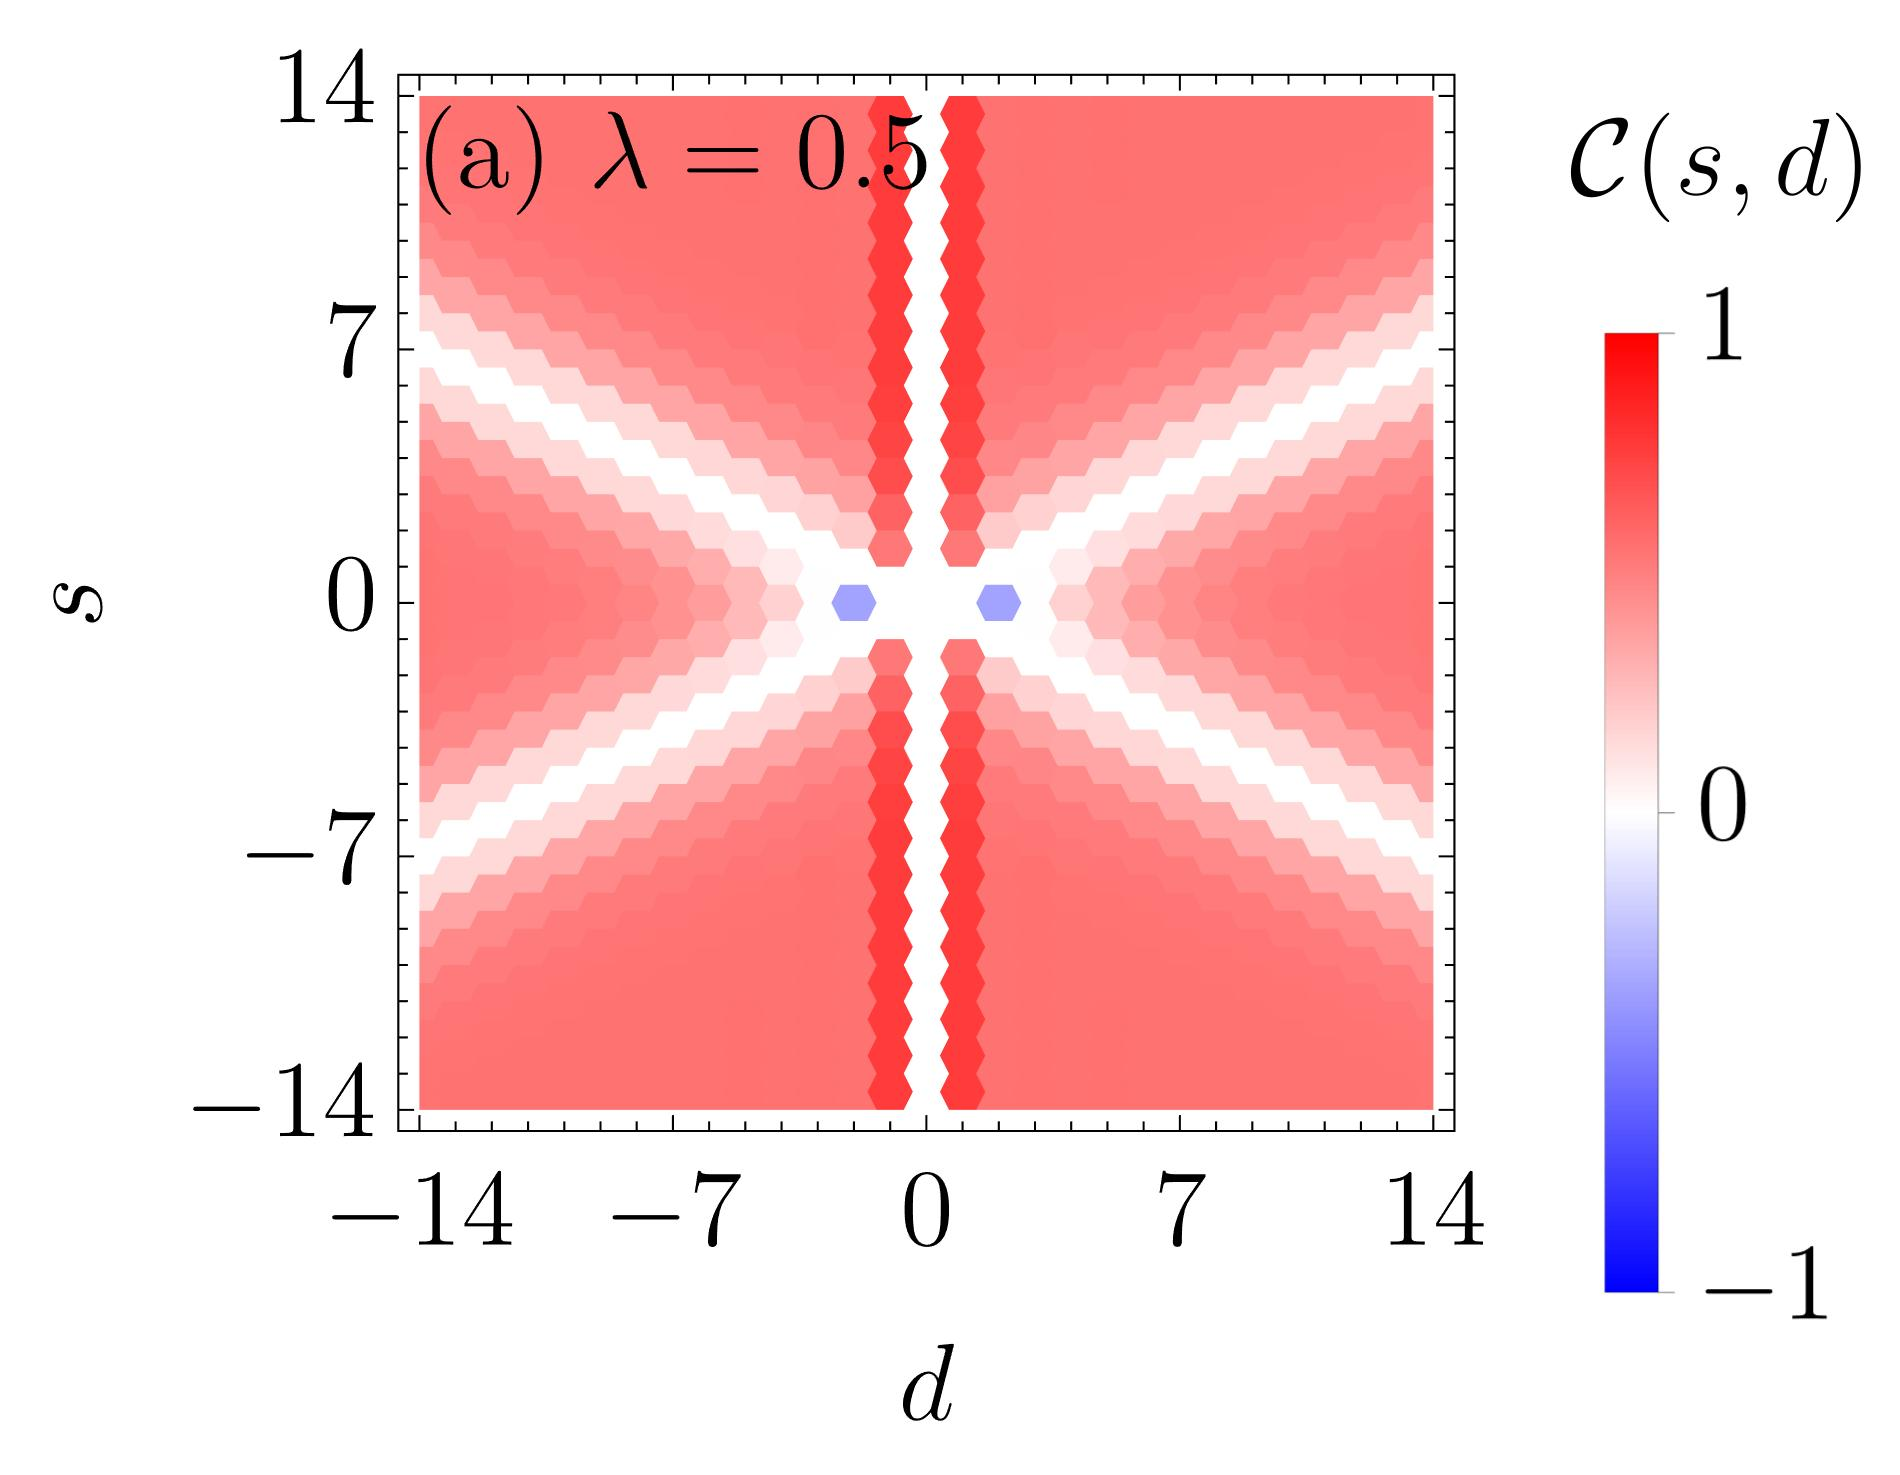
\includegraphics[width=0.32\columnwidth]{fig_5a.jpg}
	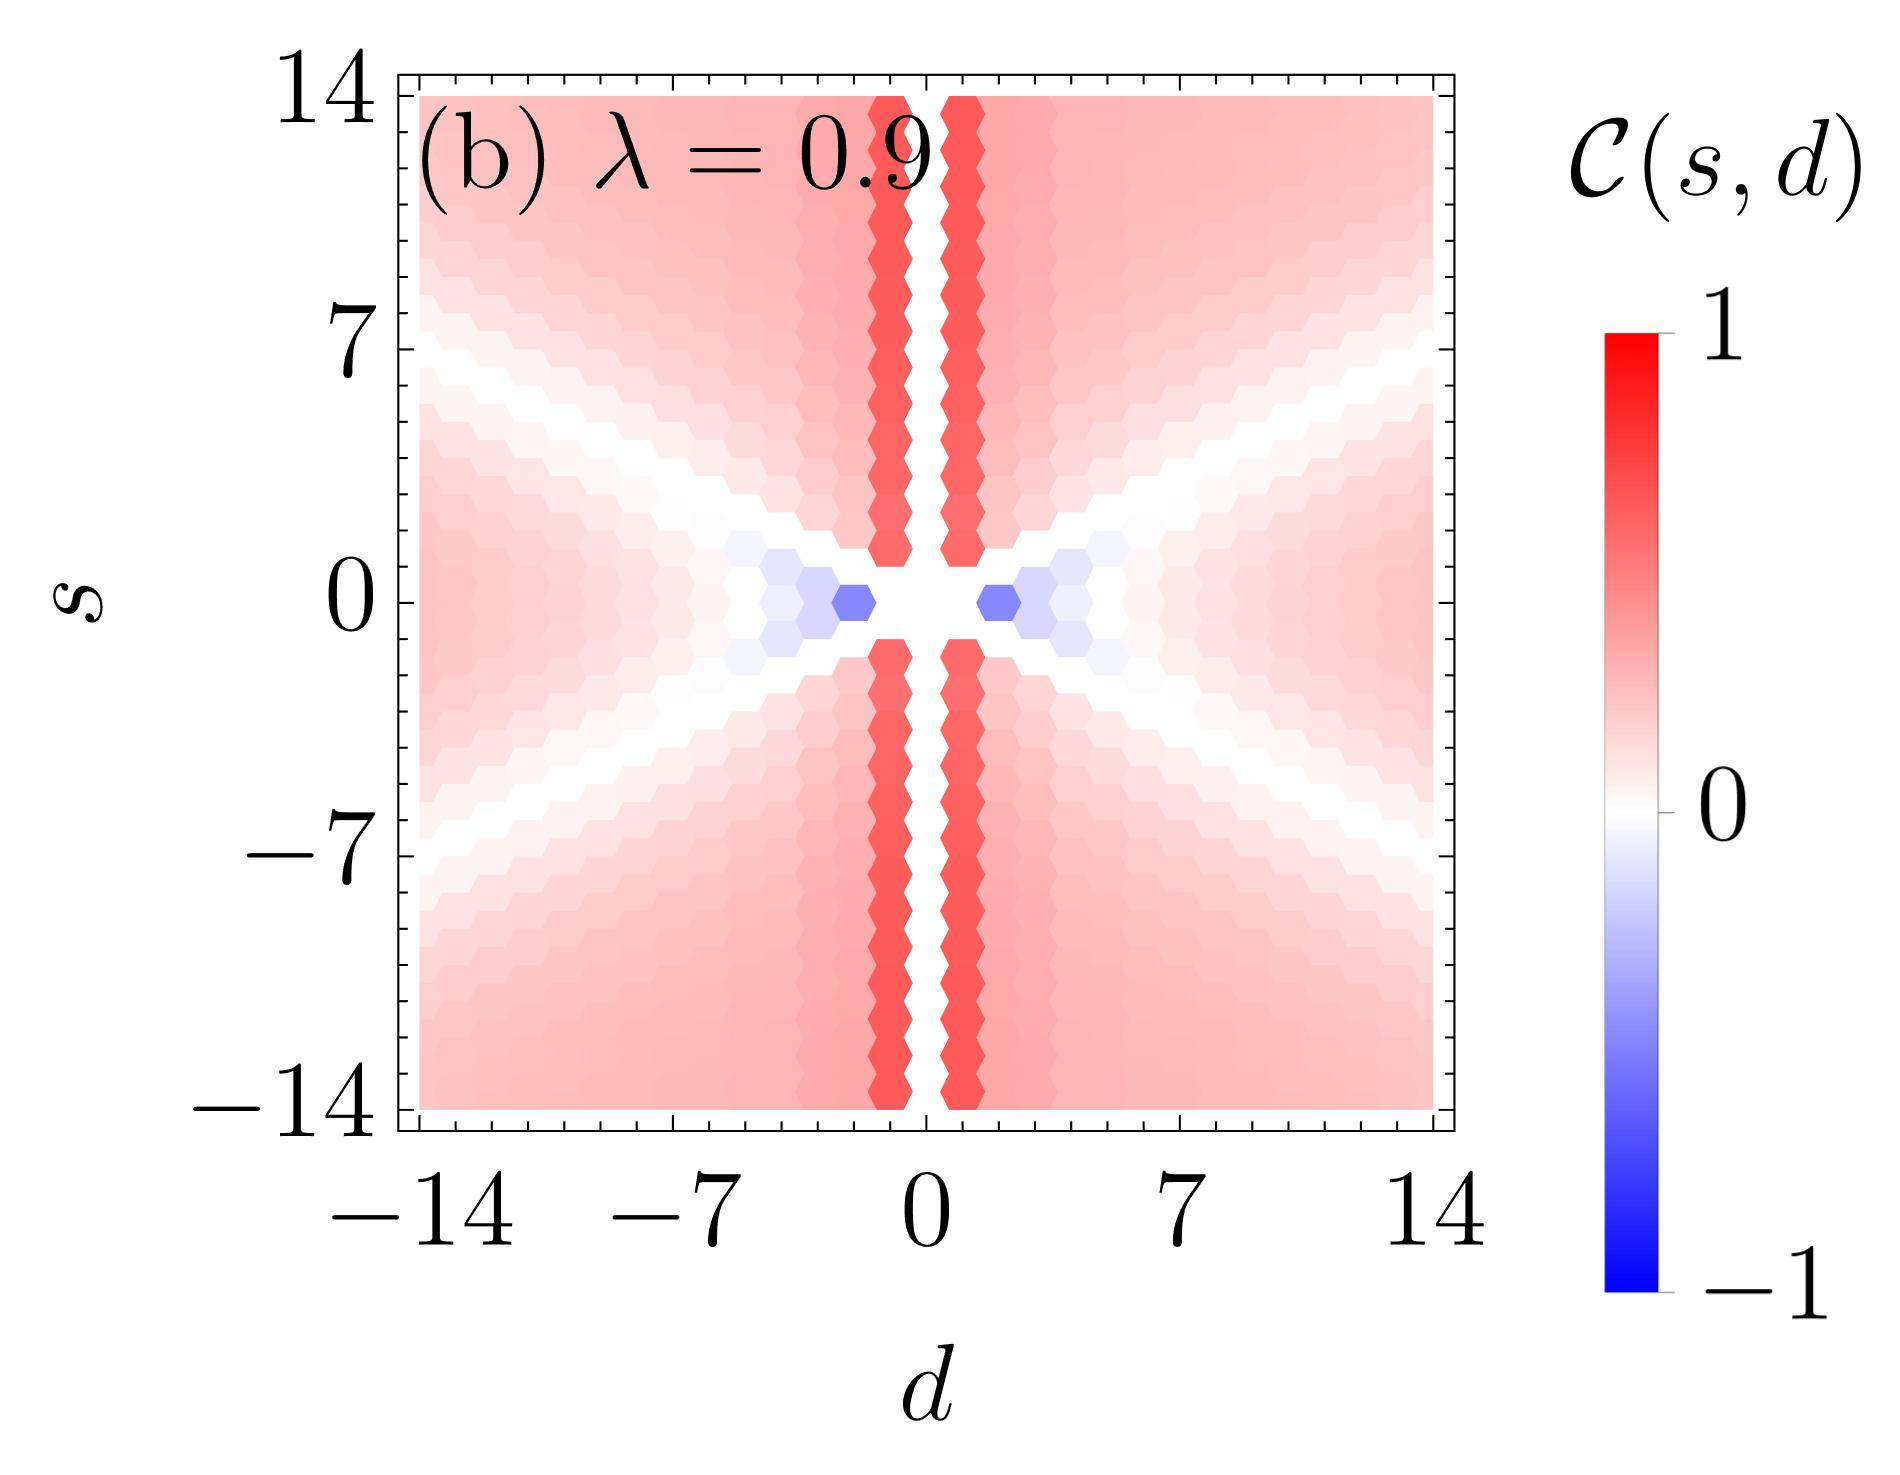
\includegraphics[width=0.32\columnwidth]{fig_5b.jpg}
	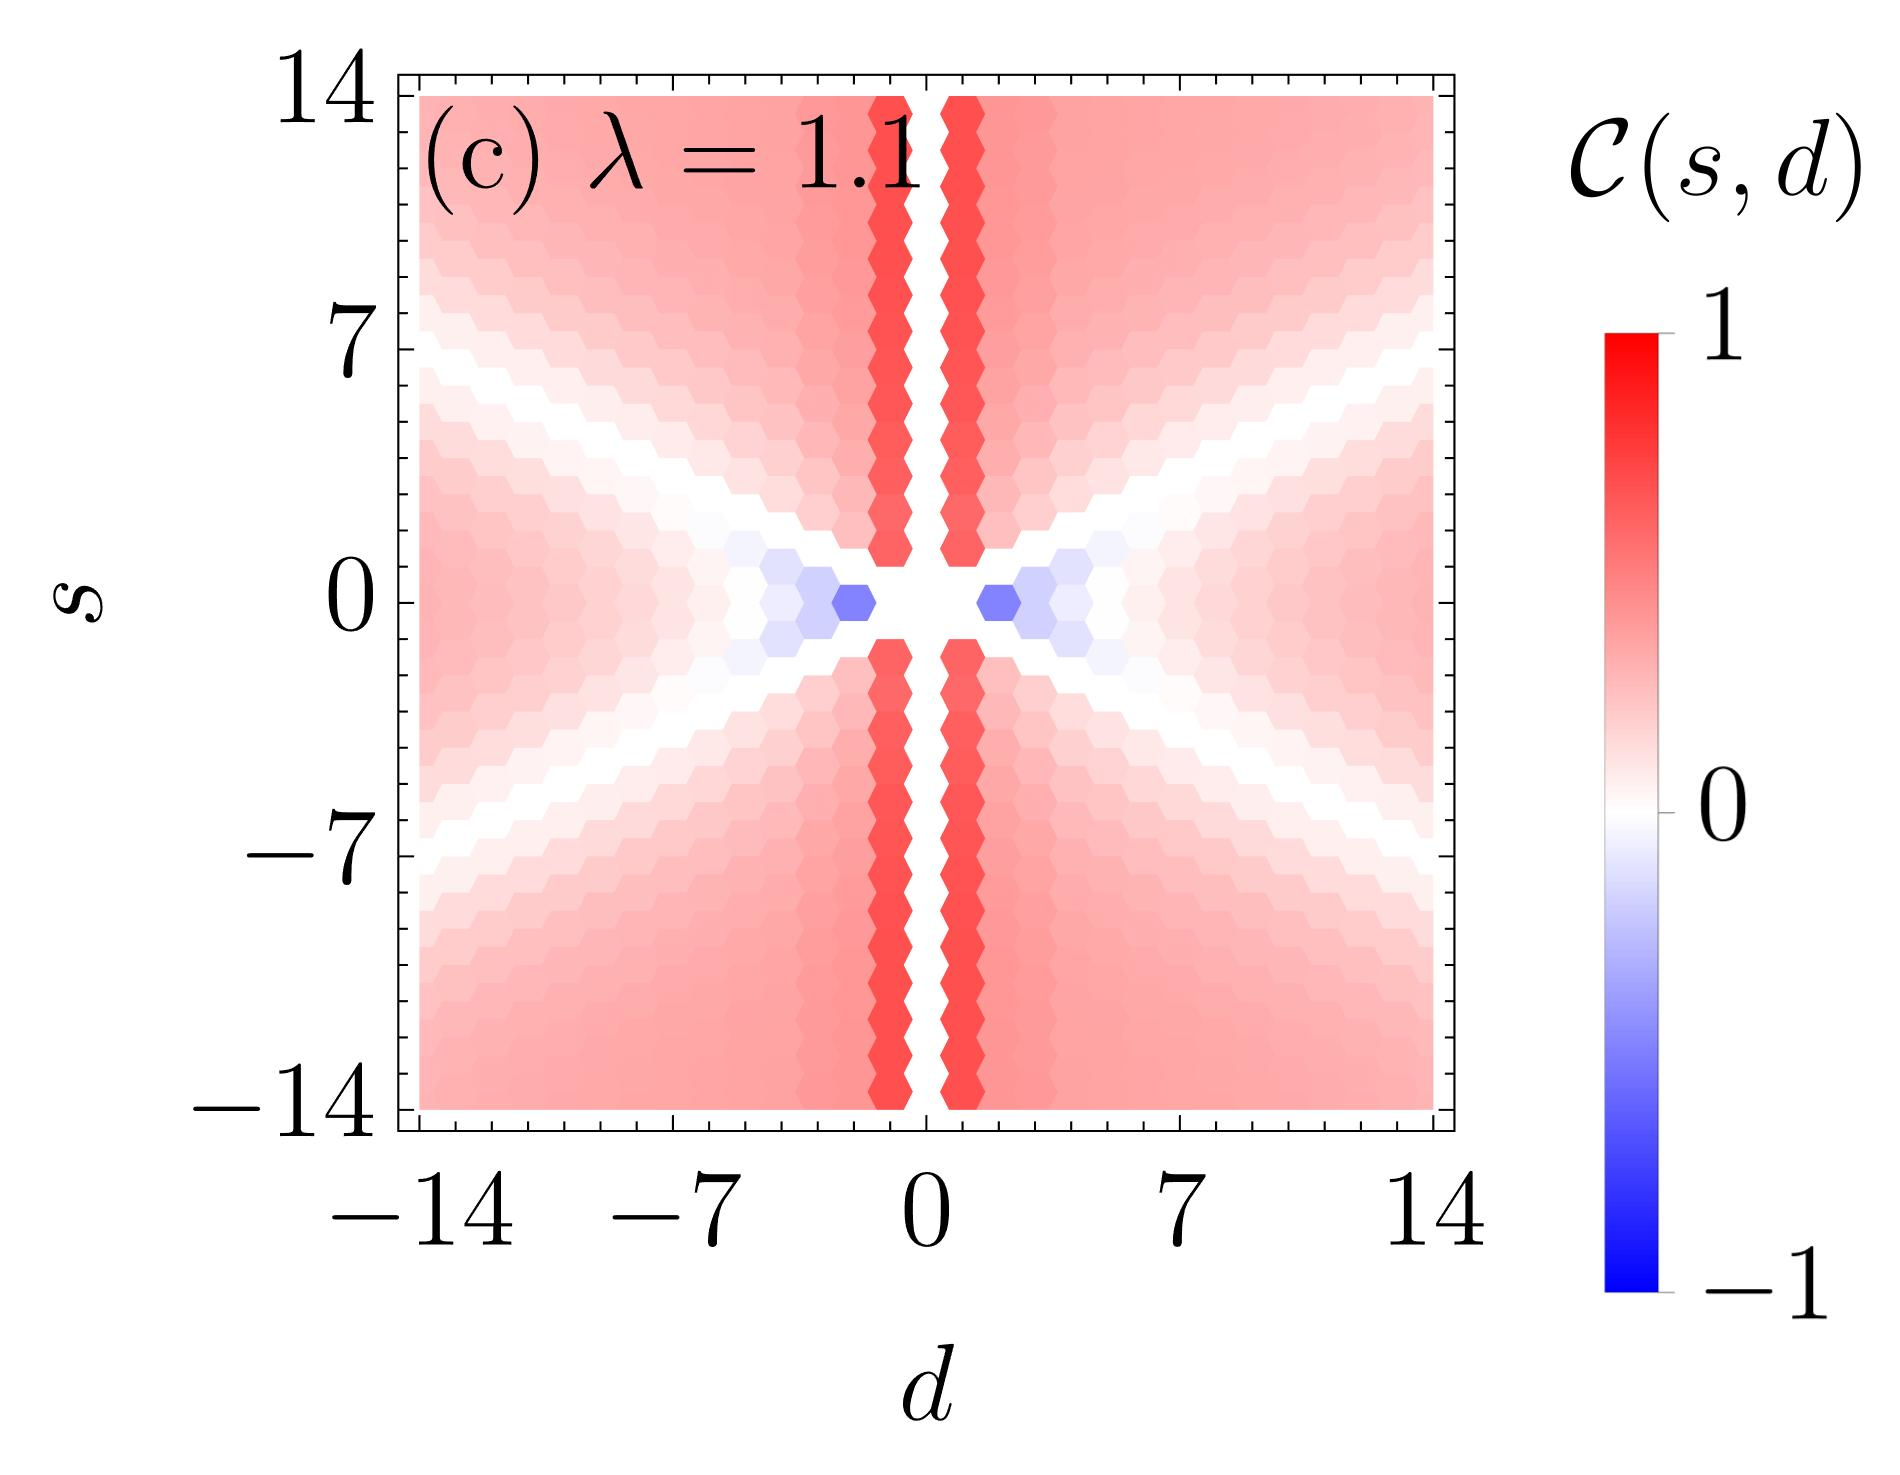
\includegraphics[width=0.32\columnwidth]{fig_5c.jpg}
  \caption{\color{red}Magnetic properties of the 1D $t$--$J$ model ground state with a single hole as probed by the hole-spin correlation function $\mathcal{C}(s, d)$: (a) with an intermediate value of magnon-magnon interactions $\lambda = 0.5$, (b-c) with the magnon-magnon interactions $\lambda = 0.9$ and $\lambda = 1.1$ close to the ideal $t$--$J$~model case ($\lambda = 1.0$). Calculation performed on the $L$~sites long periodic chain using exact diagonalization and for $J=0.4t$.
}
\label{fig:correlator_appendix}
\end{figure*}
Even for $\lambda$ close to 1, it is very clear that the cloud of magnetic excitations (flipped spins) can be observed in a small region around a hole. Such a picture is a signature of a spin polaron and it supports the claim of a breakdown of the spin-charge separation for $\lambda \neq 1$.
}

\bibliographystyle{apsrev4-1}
\bibliography{saw}

\end{document}
